\documentclass[usenames,dvipsnames,french]{beamer}

\mode<presentation> {

\usetheme{Montpellier}
}

\usepackage{graphicx} % Allows including images
\usepackage[frenchb]{babel}
\usepackage[T1]{fontenc}
\usepackage[utf8]{inputenc}
% \usepackage[demo]{graphicx}
% \usepackage{caption}

\usepackage{subcaption}
% \usepackage{subfig}
% \usepackage{algorithm,algorithmic}
\usepackage{algorithm2e}
\usepackage{listings}
% \usepackage{ntheorem}
\usepackage{booktabs} % Allows the use of \toprule, \midrule and \bottomrule in tables
\setcounter{tocdepth}{2}
\graphicspath{{../../Figures/}}


% exercices comptés
\newcounter{numexos}%Création d'un compteur qui s'appelle numexos
\setcounter{numexos}{0}%initialisation du compteur
\newcommand{\exercice}[1]{%Création d'une macro ayant un paramètre
\addtocounter{numexos}{1}%chaque fois que cette macro est appelée, elle ajoute 1 au compteur numexos
\textcolor{DarkOrchid}{Exercice\,\thenumexos\,:}\,#1%Met en rouge Exercice et la valeur du compteur appelée par \thenumeexos
}
%----------------------------------------------------------------------------------------
%	TITLE PAGE
%----------------------------------------------------------------------------------------

\setbeamertemplate{title page}{
    \centering

    \Large\bfseries
    Machine learning Tek 5: density estimation
    

\begin{figure}[!h]
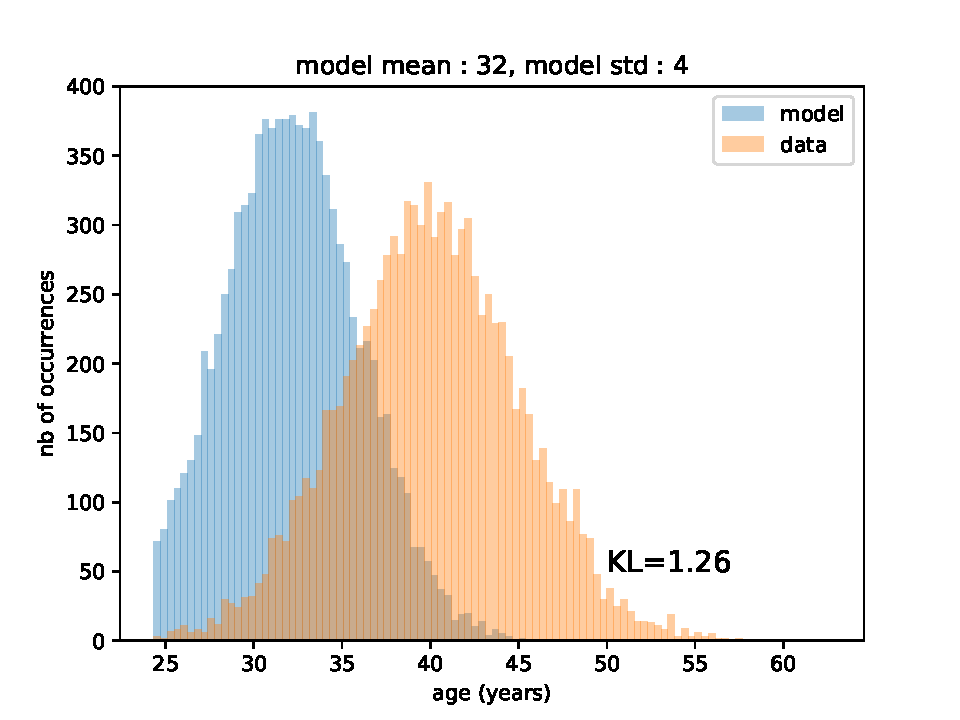
\includegraphics[width=8cm]{model_hist_mean_32_std_4.pdf}
\end{figure}

    }
\begin{document}

\frame{\titlepage}

\begin{frame}
    \tableofcontents
\end{frame}

\begin{frame}{Density estimation}

    Objective: compute a probability distribution that represents the data well.

\end{frame}

\section{Maximum likelihood}

\begin{frame}
\frametitle{Maximum Likelihood}
The \textbf{Maximum Likelihood} method is a famous method.

We observe a dataset $D_n = (x_1,...,x_n)$.

We first need to choose a \textbf{model} (which is the distribution) of the dataset, $p$.

Then, we must optimize the \textbf{parameters of this model}, noted $\theta$.
\end{frame}

\begin{frame}
    \frametitle{Maximum Likelihood}
    The \textbf{{likelihood}} (vraisemblance)  of the model is 
    \begin{equation}
        L(\theta)=p(x_1, \dots, x_n| \theta)
    \end{equation}
    Here, $p$ denotes the probability of observing the sample $(x_1, \dots, x_n)$, when the model had the parameter $\theta$, (or the probability density, in the corresponding context).
\end{frame}

\begin{frame}
    \frametitle{Maximum Likelihood}
    The \textbf{{likelihood}} (vraisemblance)  of the model is 
    \begin{equation}
        L(\theta)=p(x_1, \dots, x_n| \theta)
    \end{equation}
    This is the function that we want to \textbf{maximize}, by choosing the best possible $\theta$ (optimization problem).

    If $(x_1, \dots, x_n)$ are conditionally independant, then it writes:
    \begin{equation}
        L(\theta)=\prod_{i=1}^np(x_i|\theta)
    \end{equation}

\end{frame}

\begin{frame}
\frametitle{Remark on max-likelihood}
Most of the time it's written this way : "minimise $-log L(\theta)$"

Because the $\log$ \textbf{transforms the product into a sum}, which is easier to \textbf{differentiate}.
\begin{equation}
	-log L(\theta)=-\sum_{i=1}^{n}\log(p(x_i|\theta))
\end{equation}
\end{frame}

\begin{frame}{Example 1}
    \exercice{We observe the data $(1,0)$. We assume that these data come from a random variable that follows a Bernoulli distribution of parameter $p$. What is the likelihood of these observations as a function of $p$ ?}
\addtocounter{numexos}{-1}
\end{frame}

\begin{frame}{Example 1}
    \exercice{We observe the data $(1,0)$. We assume that these data come from a random variable that follows a Bernoulli distribution of parameter $p$. What is the likelihood of these observations as a function of $p$ ?}
    \begin{equation}
	L=P(1|p)P(0|p)
    \end{equation}
    For which value of $p$ is this likelihood \textbf{{maximum}}  ?
\end{frame}

\begin{frame}{Example 2}
    \exercice{Same question when the data $(1, 0, 1)$ is observed.}
\end{frame}

\begin{frame}{Example 3}
    \exercice{We observe the data $(2.5, 3.5)$. We assume that these data come from a normal law of parameters $\mu$ and $\sigma$.}
\addtocounter{numexos}{-1}

    What is the likelihood of $(\mu, \sigma)$ ?
\end{frame}

\begin{frame}{Example 3}
    \exercice{We observe the data $(2.5, 3.5)$. We assume that these data come from a normal law of parameters $\mu$ and $\sigma$.}
\addtocounter{numexos}{-1}
    \begin{equation}
	\begin{aligned}
	    \label{eq:}
	    L &= p(2.5|\mu, \sigma)p(3.5|\mu,\sigma)\\
	    &= \frac{1}{ \sqrt{2\pi \sigma^2} } e^{ - \frac{1}{2} ( \frac{2.5-\mu}{\sigma}   )^2 }\times \frac{1}{ \sqrt{2\pi \sigma^2}  }e^{ - \frac{1}{2} ( \frac{3.5-\mu}{\sigma}   )^2 }
	\end{aligned}
    \end{equation}
\end{frame}

\begin{frame}{Example 3}
    \exercice{We observe the data $(2.5, 3.5)$. We assume that these data come from a normal law of parameters $\mu$ and $\sigma$.}
\addtocounter{numexos}{-1}
    \begin{equation}
	\begin{aligned}
	    \label{eq:}
	    L &= p(2.5|\mu, \sigma)p(3.5|\mu,\sigma)\\
	    &= \frac{1}{ \sqrt{2\pi \sigma^2} } e^{ - \frac{1}{2} ( \frac{2.5-\mu}{\sigma}   )^2 }\times \frac{1}{ \sqrt{2\pi \sigma^2}  }e^{ - \frac{1}{2} ( \frac{3.5-\mu}{\sigma}   )^2 }
	\end{aligned}
    \end{equation}
    We wan show that the likelihood is maximum for : 
    \begin{itemize}
	\item $\hat{\mu}= \frac{2.5+3.5}{2} $
	\item $\hat{\sigma^2} = \frac{(2.5-\hat{\mu})^2+(3.5-\hat{\mu})^2}{2} $
    \end{itemize}
\end{frame}

\section{KL divergence}

\begin{frame}
\frametitle{Kullbach-Leibler Divergence}
    The KL divergence is a measure of the discrepancy between two \textbf{distributions}.
\end{frame}


\begin{frame}{Expected value (espérance)}
\begin{itemize}
    \item For a discrete random variable $X$ that takes the values $x_i$ with probability $p_i$: 
    \begin{equation}
        E(X)= \sum^{n}_{i=1} p_ix_i
    \end{equation}
    \item For a continuous random variable $X$ with density p(x): 
    \begin{equation}
        E(X)= \int xp(x)dx
    \end{equation}
\end{itemize} 
\end{frame}


\begin{frame}
\frametitle{Kullbach-Leibler Divergence}
\begin{itemize}
    \item	The samples $(x_1,..,x_n)$ are described by an empirical distribution.
    \item	The \textbf{Kullbach-Leibler divergence} is a tool to compare distributions.
    \item	It is not a distance: it is not symmetric, no triangular inequality.
\end{itemize}
\end{frame}

\begin{frame}
\frametitle{Kullbach-Leibler Divergence}
\begin{itemize}
    \item	
    \begin{equation}
        \mathcal{D}[p||q]=\mathbb{E}_{\sim  p}[\log (\frac{p}{q})]
    \end{equation}
    \item	For discrete variables
    \begin{equation}
        \mathcal{D}[p||q]=\sum_ip(i)\log \frac{p(i)}{q(i)}
    \end{equation}
    \item	for continuous variables
    \begin{equation}
        \mathcal{D}[p||q]=\int_X p(x)\log \frac{p(x)}{q(x)} dx
    \end{equation}
\end{itemize}
\end{frame}

\begin{frame}
\exercice{\textbf{Fitting a distribution}}
\addtocounter{numexos}{-1}
\begin{itemize}
    \item \textbf{cd day\textunderscore 4/density\textunderscore estimation/kl\textunderscore divergence}
    \item	A two dimensional dataset is contained in \textbf{empirical\textunderscore distribution.csv}. It represents the \textbf{{age distribution}} of some groupe of people. We want to study this age distribution.
    \item	Using \textbf{compute\textunderscore kl.py}, we will find a model $M$ such that $KL(M||\tilde{P})$ is small, with $\tilde{P}$ the empirical distribution of the data.
\end{itemize}
\end{frame}

\begin{frame}
\exercice{\textbf{Fitting a distribution}}
\begin{itemize}
    \item \textbf{First step :} choice of the model
    \item	Plot the histogram of the data : what model seems to be relevant ?
\end{itemize}
    \begin{figure}[!h]
        \centering
        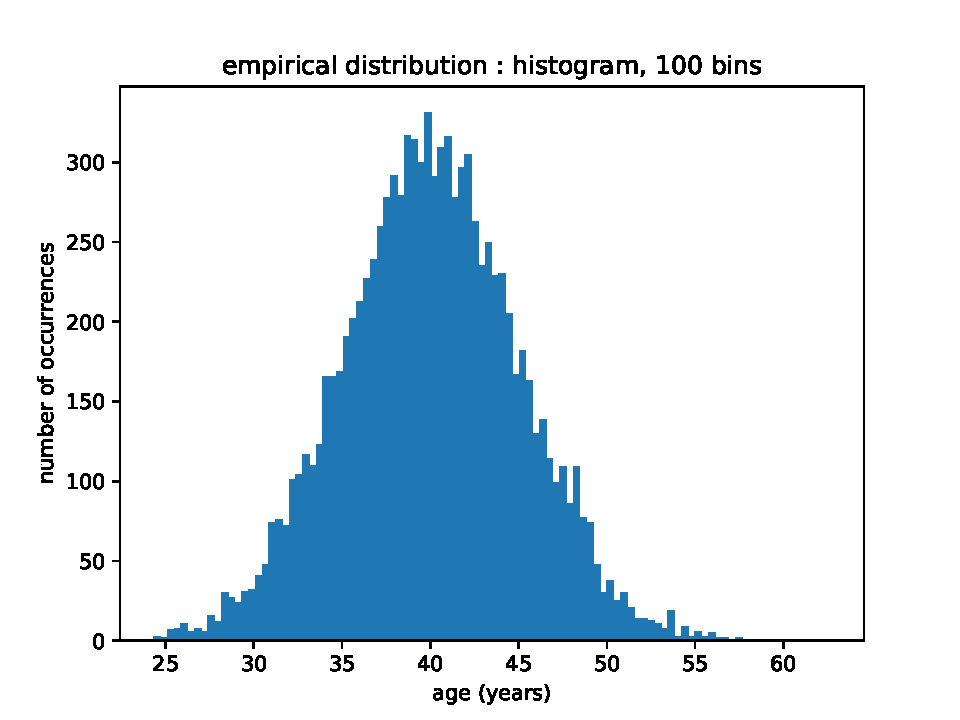
\includegraphics[width=6.5cm]{empirical_hist_100_bins.pdf}
        \label{figure}
    \end{figure}
\end{frame}

\begin{frame}
\begin{itemize}
    \item	We will use \textbf{normal laws}. We want to fit the normal law that is \textbf{the closest to the empirical data}
    \item	We measure the proximity between the model and the empirical data with the KL divergence.
    \begin{figure}[!h]
        \centering
        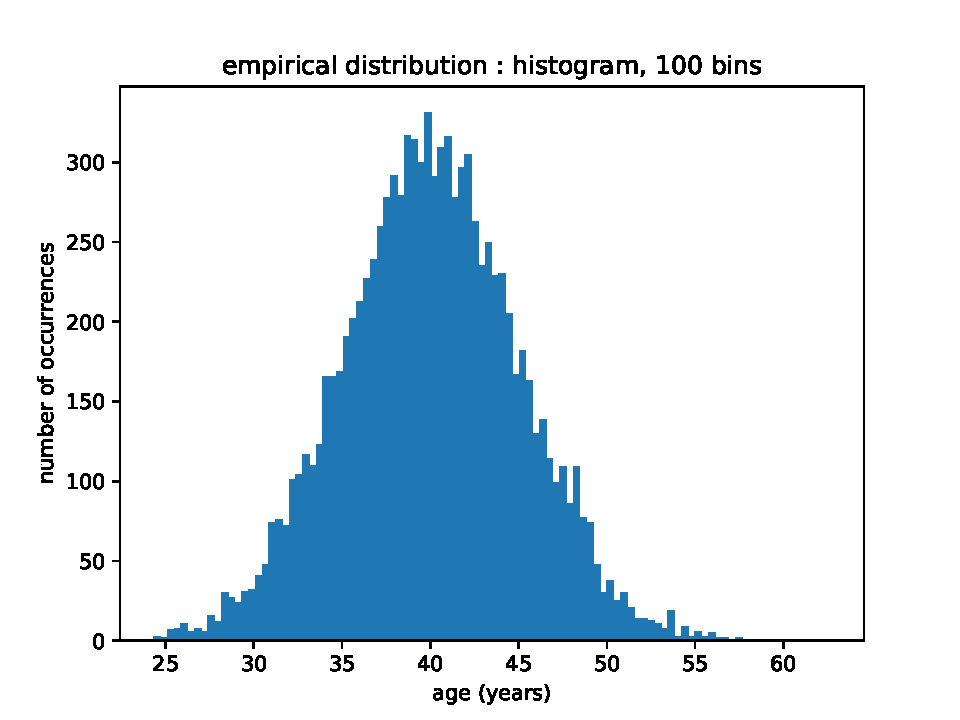
\includegraphics[width=6.5cm]{empirical_hist_100_bins.pdf}
        \label{figure}
    \end{figure}
\end{itemize}
\end{frame}

\begin{frame}
\begin{figure}[!h]
    \centering
    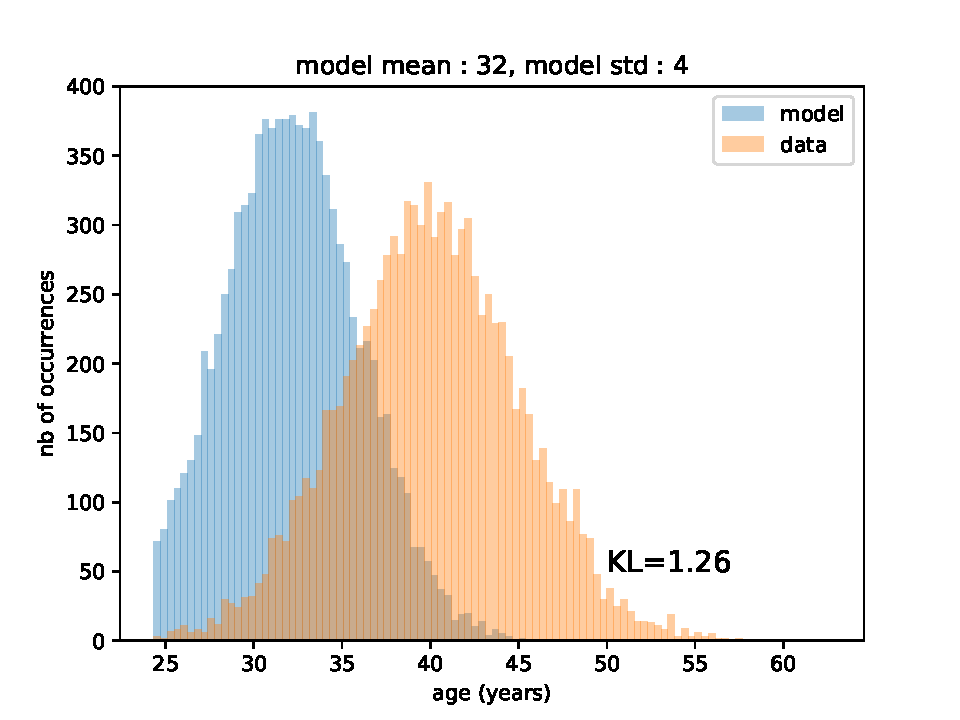
\includegraphics[width=8.5cm]{model_hist_mean_32_std_4.pdf}
    \label{figure}
\end{figure}
\end{frame}

\begin{frame}
\begin{figure}[!h]
    \centering
    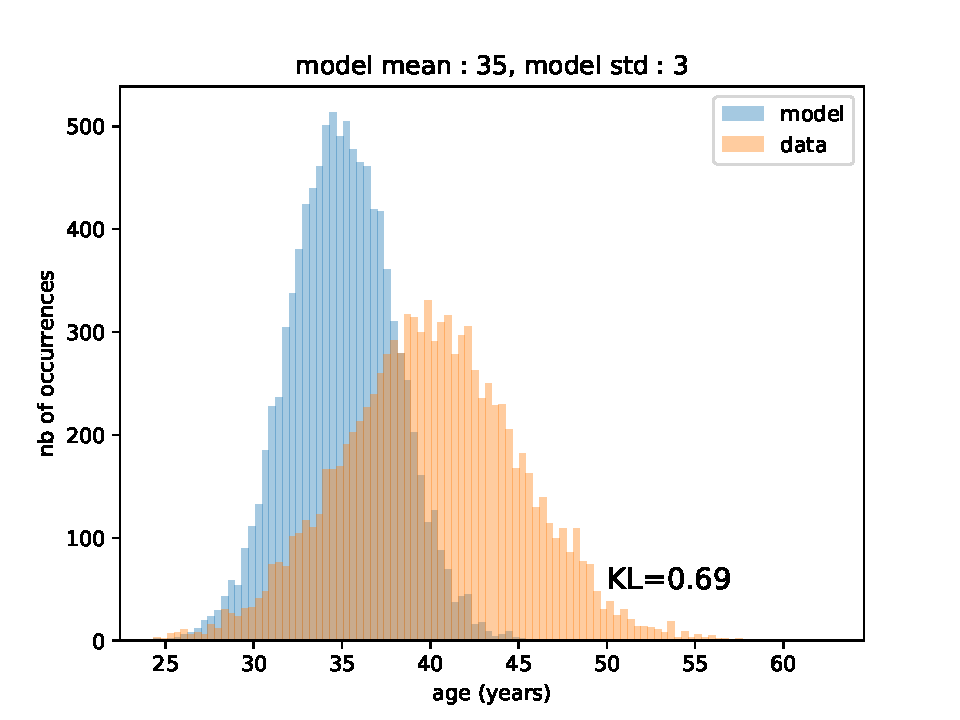
\includegraphics[width=8.5cm]{model_hist_mean_35_std_3.pdf}
    \label{figure}
\end{figure}
\end{frame}

\begin{frame}
\begin{figure}[!h]
    \centering
    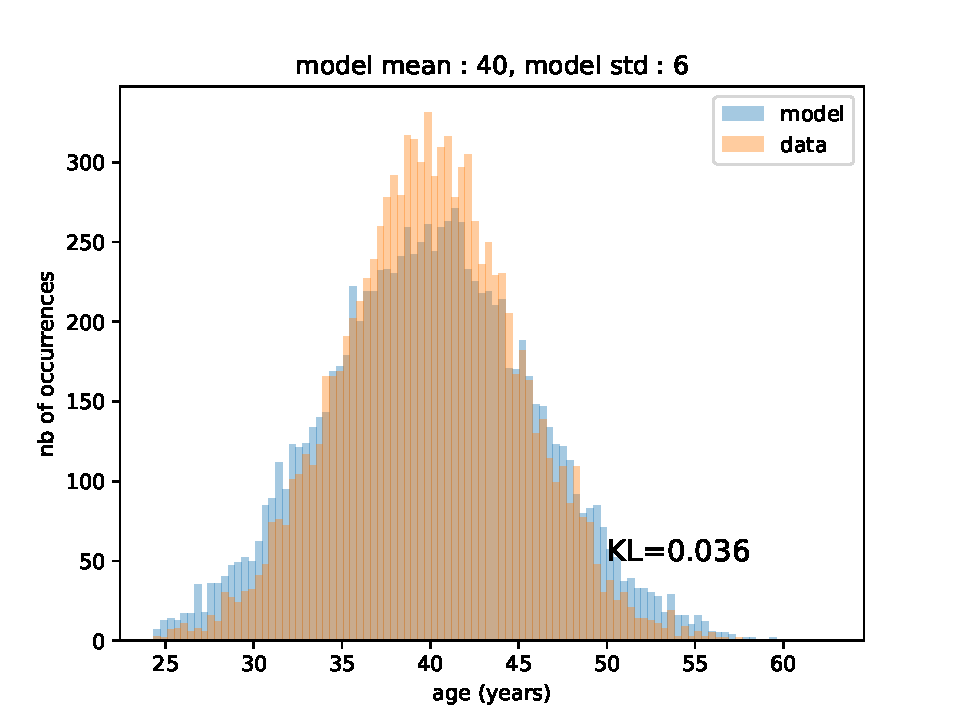
\includegraphics[width=8.5cm]{model_hist_mean_40_std_6}
    \label{figure}
\end{figure}
\end{frame}

\section{Kernel density estimation}

\begin{frame}{Kernel density estimation (non-parametric model)}
\url{https://seaborn.pydata.org/generated/seaborn.kdeplot.html} 

Example in \textbf{kde/}

\end{frame}

\begin{frame}
    \begin{figure}[htpb]
    	\centering
    	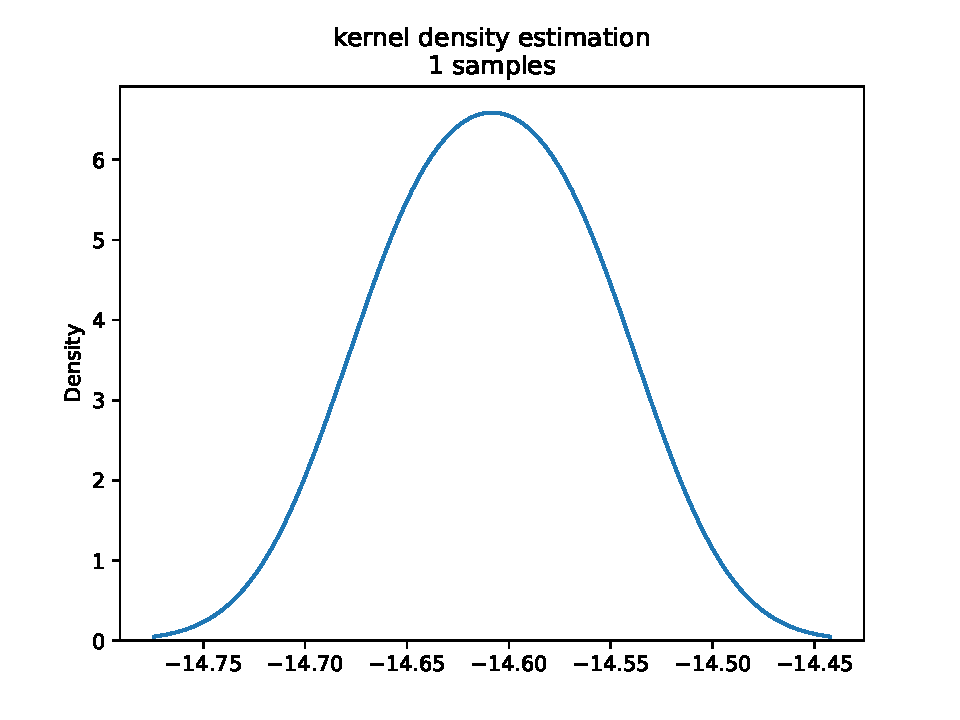
\includegraphics[width=0.8\textwidth]{kde_1_samples}
    	\label{fig:}
    \end{figure}
\end{frame}

\begin{frame}
    \begin{figure}[htpb]
    	\centering
    	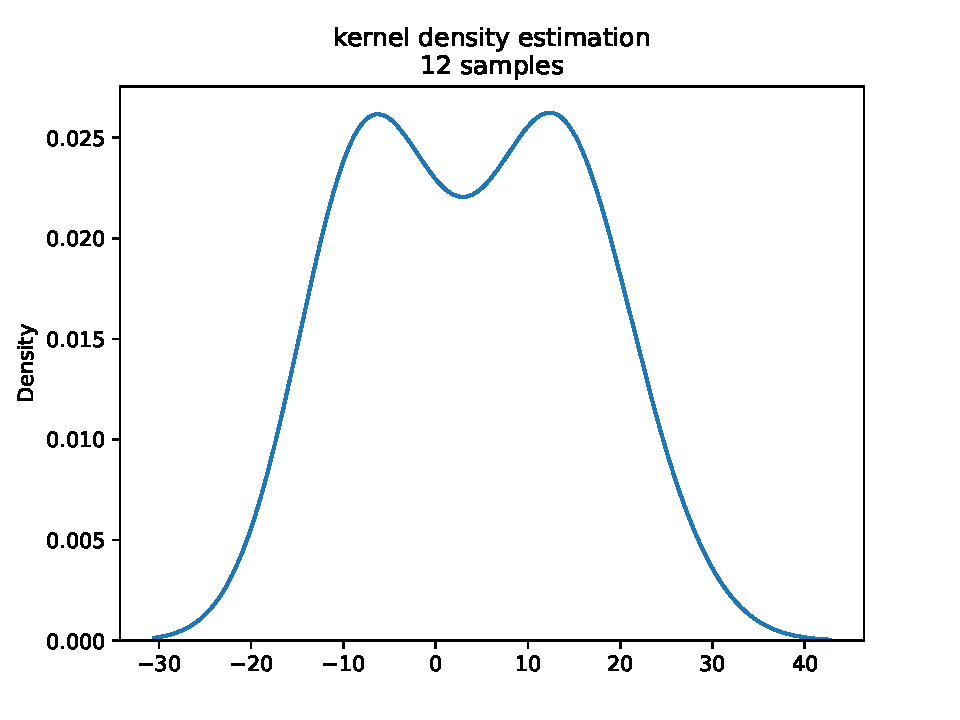
\includegraphics[width=0.8\textwidth]{kde_12_samples}
    	\label{fig:}
    \end{figure}
\end{frame}


\begin{frame}
    \begin{figure}[htpb]
    	\centering
    	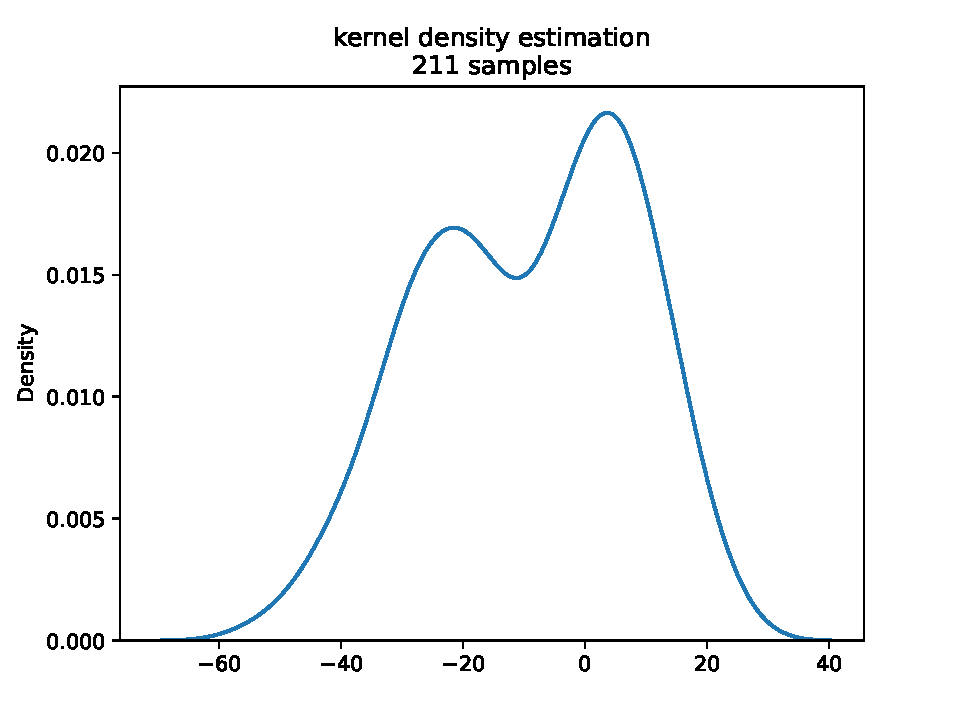
\includegraphics[width=0.8\textwidth]{kde_211_samples}
    	\label{fig:}
    \end{figure}
\end{frame}

\begin{frame}
    \begin{figure}[htpb]
    	\centering
    	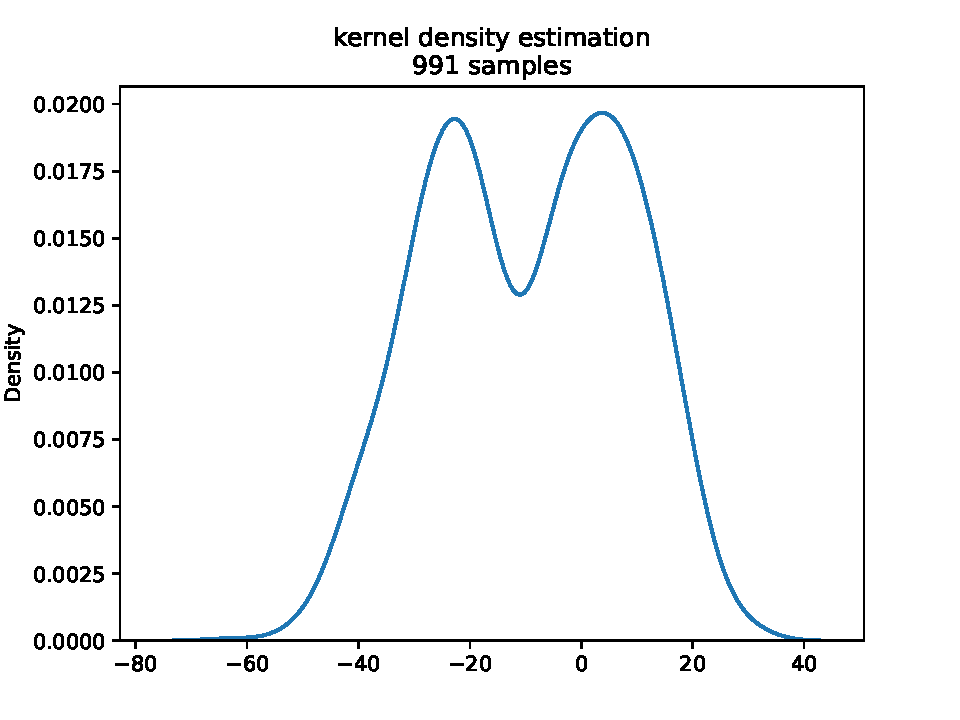
\includegraphics[width=0.8\textwidth]{kde_991_samples}
    	\label{fig:}
    \end{figure}
\end{frame}



\end{document} 
